
\subsection{Participants} 
Protocol implementation involves realization of the protocol building blocks as well as providing means of data communication between them. Building blocks are placed at the following locations, which correspond to protocol participants:

\begin{itemize}%[label=$\bullet$]
	\item User software.
	\item License Provider software.
	\item Service Provider software.
	\item License contract.
\end{itemize}

\begin{flushleft}
Data communication between protocol participants is realized in the following modes:
\end{flushleft}

\begin{itemize}%[label=$\bullet$]
	\item Transactions which change the contract state.
	\item Queries which do not change the contract state.
	\item Storing data directly in blockchain by issuing transactions.
	\item Retrieving data from blockchain by scanning transactions.
	\item Delegating ZK proof calculation.
	\item Off-chain calls.
\end{itemize}

\begin{flushleft}
The following diagram illustrates an interaction between protocol participants and indicates the communication means used.
\end{flushleft}

\begin{figure}[h]
	\centering
		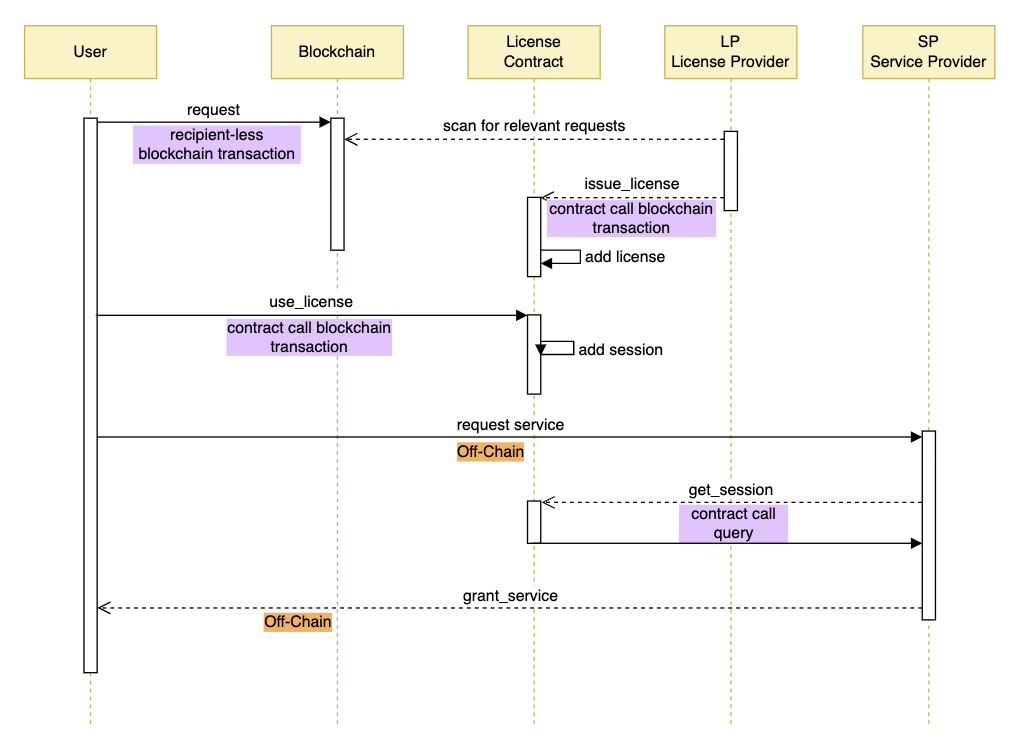
\includegraphics[width=390pt,draft=false]{images/implementation.png}
	\caption{Interaction between protocol participants}
	\label{fig:implementation}
\end{figure}

\begin{flushleft}
On the diagram, we can see various communication modes being used. Initially, user submits to the blockchain a transaction which contains request as a payload. Subsequently, License Provider can scan the blockchain for transactions containing requests and can filter out requests which are addressed to that particular License Provider. License Provider can obtain requests via other routes as well, for example via http or email, passing requests on blockchain is only one of many possible ways of submitting a request, one that has the advantage of passing a payment along with the request. Once License Provider gets a hold of a request, it can perform appropriate verification, and upon successful verification, it can issue a license. Issuing a license involves another mode of communication - a smart contract transaction call. Smart contract transaction call is also a blockchain transaction, yet to not confuse the reader, we show it on the diagram while omitting the details of blockchain involvement. The user obtains licenses via a contract query. For privacy reasons, the user obtains a bulk of licenses not pertaining exclusively to her, and she filters it out by herself. To economize the volume of data transfers, block-height range is passed to allow for a transfer which includes only a subset of available records. All modes of communication used so far were on-chain. Communication between the user and ServiceProvider, on the other hand, is off-chain. When Service Provider wants to establish a session, it calls a contract to obtain a session for a given session id.
\end{flushleft}

The diagram illustrates the following flow of data and interactions between participants:

\begin{itemize}%[label=$\bullet$]
	\item User submits request to a License Provider by issuing blockchain transaction.
	\item License Provider scans the blockchain and obtains the request.
	\item License Provider, upon necessary verification, issues a license.
	\item License Provider sends license to the License Contract via a smart contract call transaction.
	\item User obtains licenses for a given block-height range.
	\item User filters out licenses addressed to her/him.
	\item User calculates a proof (the proof calculation might be delegated).
	\item User calls \textit{use-license} to redeem a license, via a smart contract call.
	\item License Contract attempts to verify the proof and, if verified, adds a new session to a list of sessions.
	\item User requests a service from a Service Provider (off-chain).
	\item Service Provider asks contract for a session.
	\item Service Provider grants service to the user (off-chain).
\end{itemize}


\subsection{License Contract}

\begin{flushleft}
License contract maintains state consisting of the following data:
\end{flushleft}

\begin{itemize}%[label=$\bullet$]
	\item List of sessions.
	\item Map of licenses and their positions in the Merkle tree.
	\item Merkle tree of license hashes.
\end{itemize}


\begin{flushleft}
Contract provides the following methods:
\end{flushleft}

\begin{itemize}%[label=$\bullet$]
	\item \textit{issue-license}: adds a license to a Merkle tree of licenses.
	\item \textit{get-licenses}: provides a list of new licenses added in a given block-height range.
	\item \textit{use-license}: attempts to verify the proof and, if verified, adds a new session to a list of sessions and nullifies the license in the Merkle tree.
	\item \textit{get-session}: finds a session in a list of sessions and returns it to the caller.
\end{itemize}


\subsection{License ZK Proof Calculation}

License ZK proof calculation will either be performed by the user or delegated to a node. At the time of writing, the details of delegation are not known yet, they will be filled in here once the information becomes available.
